% Chapter 5

\chapter{Galaxy Pairs, Mergers, and Morphologies} 
\label{Chapter:GalPairs}
\lhead{Chapter 5. \emph{Pairs, Mergers, and Morphologies}} 

\section{Background}

$\Lambda$CDM cosmology predicts the hierarchical assembly of dark matter haloes.
Throughout the history of the Universe haloes have grown in mass and size via two pathways. 
Firstly haloes grow via smooth accretion gradually accreting dark matter from the surrounding environment. 
The secondary growth mechanism is via the accretion and gradual absorption of smaller haloes, known as subhaloes. 
After accretion subhaloes survive as substructure of the central/host halo gradually losing mass and sinking to the centre of the potential well though dynamical friction. As discussed in previous Chapters these sub-haloes contain satellite galaxies that follow the halo structure resulting in galaxy galaxy mergers.

Frequent or massive mergers are thought to induce morphological changes in galaxies. 
Galaxies, after experiencing a massive merger, where the minor galaxy is at least a quarter of the mass of the central galaxy, are thought to lose their disk-like morphology and transform into elliptical galaxies \citep{Negroponte1983SimulationsGalaxies, DeLucia2006TheGalaxies}. 
For this reason it is important to understand the frequency and nature of mergers between galaxies to achieve a complete and coherent picture of galaxy formation and evolution. 
Unfortunately, galaxy mergers occur on gigayear timescales and therefore it is not possible to directly observe the rate or consequence of galaxy mergers. 
The traditional approach to estimate the rate of galaxy mergers is to count galaxy pairs, and then assign a merging timescale to infer the rate \citep{Conselice2003A3,Conselice2008TheField,Mundy2017A3.5,Duncan2019ObservationalFields}.
A galaxy pair is usually defined by a mass ratio and a separation, for example we may be looking at galaxies that are within 5 to 30 kpc and would fit the major merger criteria (1/3 mass ratio).
However, the approach of counting pairs is complicated by systematic differences when selecting galaxies. For example, the evolution of the pair fraction appears to change if a selection is made by flux ratio or made by stellar mass ratio \citep{Man2016RESOLVING03}.

\section{The systematic effects of stellar mass estimation on galaxy pair fractions}

%What systemeatics can we expect to find in galaxy pairs (paper 3 plots 1,2,&3)

In this chapter we show how different SMHM relations generate distinct pair fractions and by association different merger rates. 
Stellar mass functions with greater number densities of high-mass galaxies map larger galaxies into smaller haloes, resulting in steeper high-mass slopes for the SMHM relations.
In Figure \ref{fig:MassRatioCartoon} we show an illustrative cartoon of how different SMHM relations affect the galaxy mass ratios. 
For two identical halo pairs we see that a SMHM relation with a steeper slope causes a substantial difference in the stellar mass ratio that is mapped into the halo pairs when compared to a shallower SMHM relation. 

\begin{figure}[h]
	\centering
	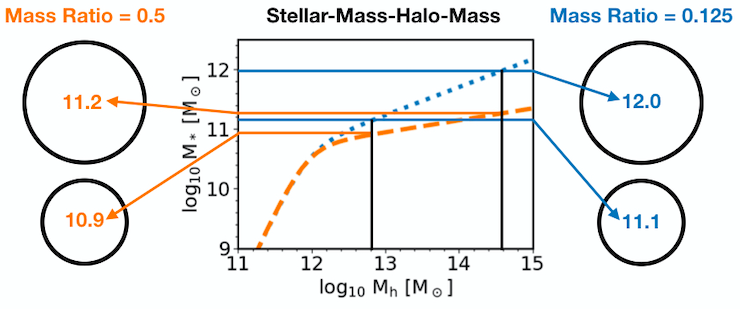
\includegraphics[width = \linewidth]{Figures/Chapter5/MassRatioCartoon.png}
	\caption{A cartoon showing the how the SMHM relation can impact the stellar mass ratio of galaxies mapped into identical halos. The steeper SMHM relation creates a smaller stellar mass ratio as the change in halo mass maps to a much larger stellar mass difference.}
	\label{fig:MassRatioCartoon}
\end{figure}

It follows that given two identical distributions of haloes seeded with galaxies via different SMHM relations the shallower one will seed more galaxy pairs\footnote{The pair fraction defined here as the fraction of galaxies of a given mass that have a companion with a mass equal to or greater than a quarter of the primaries mass within 5-30 kpc.}.

In Figure \ref{fig:SMHM_PF_Cartoon} we show an example of systematic difference expected in the pair fraction when changing the SMHM relation.
The left hand column shows the SMHM relations and the right column the pair fractions and their evolution with redshift. 
In the top row we compare two high mass slopes one steep one shallow, where the slope has been changed at fixed redshift $z = 0.1$.
In the bottom row we compare an evolving and non-evolving high-mass slope.

\begin{figure}[h]
	\centering
	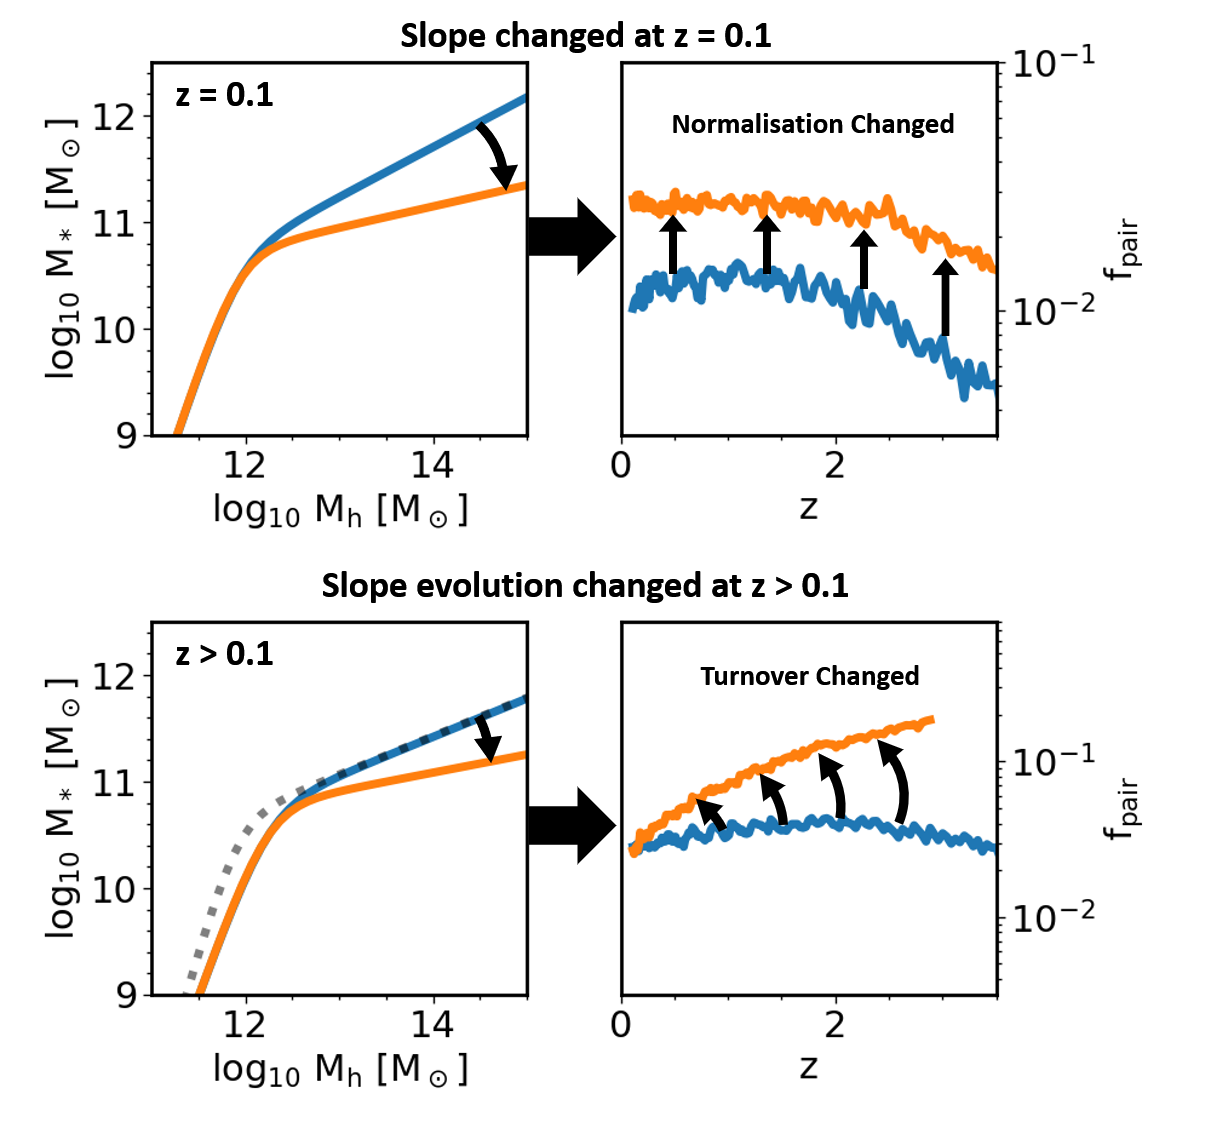
\includegraphics[width = \linewidth]{Figures/Chapter5/SMHM_PF_Cartoon.png}
	\caption{A cartoon showing the how the SMHM relation can impact the pair fraction. The top row shows how reducing the high mass slope of the SMHM relation increase the number of pairs at all redshifts. The bottom row shows the redshift $z=0.1$ relation as a grey dotted line alongside two evolving relations at redshift $z=2$ where one relation is evolved to be shallower shown in orange respectively compared to the relation in blue that remains steeper. For the SMHM relation that evoloves to be shallower the pair fractions are found to increase. In each case the reason for the increase can be explained by referencing Figure \ref{fig:MassRatioCartoon} where making the relation shallower seeds more massive pairs.}
	\label{fig:SMHM_PF_Cartoon}
\end{figure}

The suppression of the high-mass slope increases the number of pairs created and the normalisation of the pair fraction increases. 
In the bottom row we show the effects of having a slope that flattens at higher redshift. 
We show the redshift $z=0.1$ relation in grey and the relations with the unchanged and changed slopes in blue and orange respectively. 
The main effect of varying the evolution of the high-mass slope in the SMHM relation is to change the behaviour of pair fraction with redshift. 
A steeper slope leads to a decreasing pair fraction and whereas a slope that gets shallower with time results in an increasing pair fraction.


The behaviours reported in Figure \ref{fig:SMHM_PF_Cartoon} are what one would expect given Figure \ref{fig:MassRatioCartoon}, where shallower slopes give higher fractions. 
Furthermore, from Figure \ref{fig:SMHM_PF_Cartoon} (and from Figure \ref{fig:PairFracSystematic}), it can be concluded that almost any pair fraction difference could be produced by appropriately altering the input SMHM relation. 
It is relevant to stress here that relatively minor changes in the stellar mass function can cause qualitative differences in the SMHM relation and, by extension, in the shape and normalisation of pair fractions at any cosmic epoch.

The ability to systematically change the pair fraction due to stellar mass derivation calls to question the discrepancies found in pair fraction results \citep[e.g.][]{Man2016RESOLVING03}. 
If the pair fraction is systematically effected then where results do not use the same data processing then any differences could be due to non-trivial systematics. 
\steel as a flexible and lightweight model can illuminate the systematics by running with multiple input SMHM relations to test a range of different inputs and compare the results.

Calculation of the pair fraction in \steel requires an estimate of the distance between the central galaxy and the satellite galaxy. Using statistical accretion histories we do not have discrete halos and therefore lack `physical' separations, we instead assign each subhalo bin an average distance to the central galaxy. 
The subhaloes start at the viral radius of the central halo, the distance to the centre then reduces proportionally to the amount of dynamical time remaining \citep{Guo2011FromCosmology}.

In this chapter we investigate the distribution of satellites around central galaxies when using different SMHM relations. This distribution is primarily dominated by the halo substructure, for this reason it is essential to make sure our selection criteria for galaxies always returns the same halo population. As we actively change the stellar masses mapped into any given halo mass one cannot use a stellar mass cut to achieve this result. From a simulation where the haloes are known, one could simply select by halo mass, however, to better match observation, where haloes are not known, we make a constant number density selection. A constant number density selection will always return objects that share a given number density and are therefore associated to the same haloes, as we assume the halo structure is a fixed quantity. A similar technique was employed by, \citet[e.g.][]{Leja2013TRACINGSELECTION, Mundy2015Tracing3} to trace the evolution of galaxy populations; galaxies at high redshift with a given co-moving number density are assumed to be the progenitors of later populations with the same abundance. 
In this work we use a central stellar mass selection from the PyMorph stellar mass estimation of $M_{*} = 10^{11} - 10^{11.6} M_{\odot}$ (or $10^{9.5} - 10^{10.1} M_{\odot}$ when considering the low-mass slope controlled by $\beta$). The number-density range of the aforementioned mass cut is then computed and galaxies are selected from the other SMHM relations which share this number density.
An example of this selection can be seen in Figure \ref{fig:PairFracSystematic}, the shaded horizontal band shows the stellar masses for each SMHM relation that share number density.

The SMHM relation is defined by 4(+4) parameters, we build a toy model where each of the parameters (M, N, $\beta$, $\gamma$), and their evolutionary factors (M$_z$, N$_z$, $\beta_z$, $\gamma_z$), are adjusted in turn to explore the affect on the galaxy pair fractions. Table \ref{tab:PairFracSysInput} details the change made to the SMHM relation for each parameter. 

\begin{table}
\centering
\caption{The adjustments to the SMHM relation used in Figure \ref{fig:PairFracSystematic}.}
\label{tab:PairFracSysInput}
\begin{tabular}{|c|cccc|} \hline
             & PyMorph   & $X_{0.1, alt}$  & $X_{z, +}$  & $X_{z, -}$  \\ \hline
$M$          & 11.92 & -0.25 & -     & -     \\ 
$M_{z}$      & 0.58   & -     & +0.1  & -0.1  \\ \hline
$N$          & 0.032 & +0.04 & -     & -     \\
$N_{z}$      & -0.014 & -     & +0.007 & -0.007 \\ \hline
$\beta$      & 1.64  & -0.3  & -     & -     \\
$\beta_{z}$  & -0.69  & -     & +0.3  & -0.3  \\ \hline
$\gamma$     & 0.53  & +0.06 & -     & -     \\
$\gamma_{z}$ & -0.03  & -     & +0.2  & -0.2  \\ \hline
\end{tabular}
\end{table}

Figure \ref{fig:PairFracSystematic} shows each of the SMHM relations in the outer four panels, the reference SMHM relation PyMorph is shown in blue at redshifts $z = 0.1$ (dotted line) and $z = 2$ (dashed line) in each panel, the modified redshift $z = 0.1$ relation is then shown in orange, and the increased and decreased (dashed red and green) evolution relations are shown at redshift $z = 2$. The inner four panels show the results on the pair fraction and follow the same colour convention. 

\begin{landscape}
\begingroup
\begin{figure}[h]
	\centering
	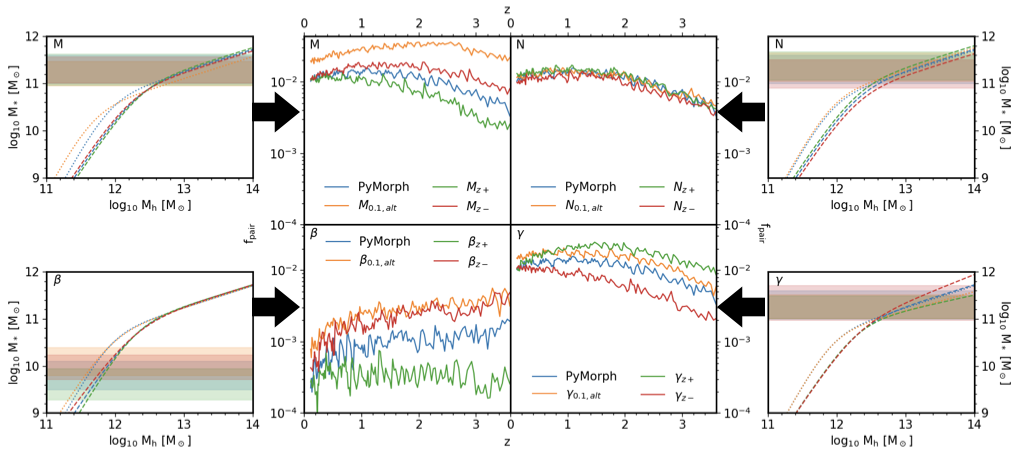
\includegraphics[width = \linewidth]{Figures/Chapter5/PairFractionSystematic.png}
	\caption{Each of the panel pairs (M, N, $\beta$, $\gamma$) shows the input SMHM relation in the outer plot and the modelled pair fraction evolution in the centre plot. Each pair investigates adjustments to the given parameter of the SMHM relation (M, N, $\beta$, $\gamma$). Each pair shows the reference SMHM relation `G18' in blue, the relation adjusted at redshift $z = 0.1$ keeping the same SMHM relation evolution parameters in yellow. The red and green lines have the evolution parameter altered such that the evolution parameter is increased or decreased with respect to PyMorph respectively. In the outer (SMHM relation) plots dotted lines are $z = 0.1$ relations and dashed lines are $z = 2$ relations, the PyMorph relation is shown at both epochs for comparison. Finally the shaded bands in the outer plots show the consistent number density selections used in the centre plots.}
	\label{fig:PairFracSystematic}
\end{figure}
\endgroup
\end{landscape}

When changing M, the knee parameter, a large increase in the pair fraction is found from a lower knee: The shallower high mass slope is extended, therefore more haloes are seeded in the mass range for pair selection. 
We see the same effect at high redshift, the lower value of M creates a higher pair fraction. 
The normalisation parameter, N, creates little change in the pair fraction as expected because the mass ratios are largely unaffected. 
The low mass slope parameter, $\beta$, affects the seeding of smaller galaxies hence a lower mass range is used for the consistent number density cut. 
Due to the steepness of the low mass slope the fraction of pairs found is lower in this mass cut.
Finally, when the high mass slope parameter, $\gamma$, is altered more pairs are found at high and low redshift when the slope is shallow. 
This is again attributed to more galaxies seeded within the mass ratio range.

\subsection{Comparison to simulation and observational Results}
\label{subsec:SimObsRes}
The observed pair fraction is known to have discrepancies based on the galaxy property used to calculate the ratio. In \citet{Man2016RESOLVING03} it is shown that selecting pairs by flux ratio or stellar mass creates differences in the pair fraction evolution. 
In Figures \ref{fig:MassRatioCartoon} \& \ref{fig:SMHM_PF_Cartoon} we show the predicted effect of the determination of stellar mass on the SMHM relation and the systematic propagation of these changes into the pair fraction. 
Through the use of a toy model in Figure \ref{fig:PairFracSystematic} we show how isolated perturbations to the eight SMHM relation parameters propagate into the galaxy pair fraction.
Given this analysis we find that any observation of the pair fraction must be understood in terms of its implicit observational assumptions. 
Furthermore, direct comparison of pair fraction results should only be undertaken under identical stellar mass derivation assumptions, or where this is not the case the influence of any differences are accounted for.
In this section we fit, by making use of $\steel$, observed pair fractions using small changes to the SMHM relation.
We anticipate this modelling can be used to provide corrections to pair fraction results to allow for fairer comparisons.

In Figure \ref{fig:PairFractionIll} we show the simulated galaxy pair fractions for galaxies in the mass range $M_*$ = $10^{10}$ to $10^{10.6}$. The pair fraction is shown for two different SMHM relation inputs to $\steel$. In blue we show the PyMorph (S\`ersic Exponential) input used as the baseline in Figure \ref{fig:PairFracSystematic}, in orange the input SMHM relation is calibrated to match the Illustris TNG simulation. In the right hand panel we see that the the prediction from \steel with the TNG-calibrated input is in good agreement to the pair fraction extracted directly from the Illustris TNG simulation. The pair fraction predicted using the PyMorph input is 0.5 dex lower, this is to be expected as in the mass range we are considering the Illustris TNG simulation SMHM relation is shallower and more pairs are therefore created in a greater mass range of halo mergers. 
\begin{figure*}
	\centering
	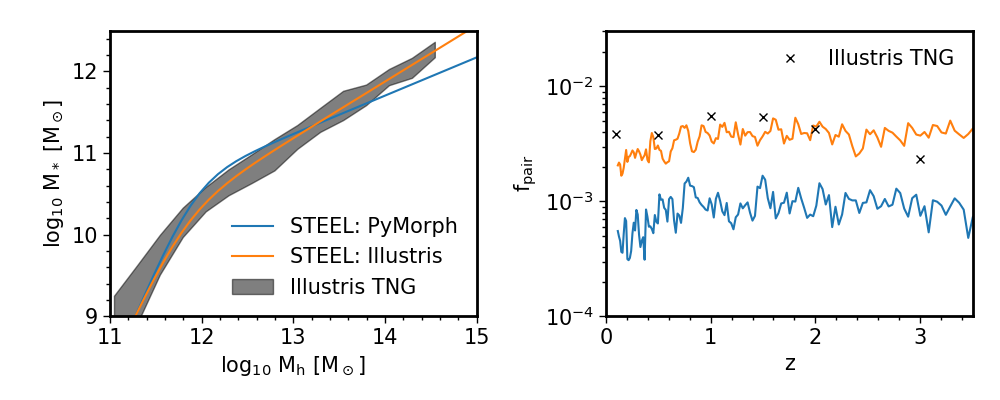
\includegraphics[width = \linewidth]{Figures/Chapter5/PairFractionIllustris.png}
    \caption{Left: Two SMHM relations are shown from \steel using parameters designed to reproduce the SMHM relation found in the Illustrius TNG simulation (Orange line) and the PyMorph(S\`ersic Exponential) fit parameters (Blue line). The shaded region is the output from the Illustris TNG simulation. Right: The pair fraction, for galaxies in the mass range $M_*$ = $10^{10}M_{\odot}$ to $10^{10.6}M_{\odot}$ is shown both the SMHM relations. Lines are the output from \steel following the same colours as the left hand panel. The pair fraction extracted directly from the Illustris TNG simulation is shown using black crosses.}
	\label{fig:PairFractionIll}
\end{figure*}

Figure \ref{fig:PairFractionData} shows the predicted pair fraction evolution using the two SMHM relations from PyMorph and cmodel presented in Section \ref{C2:SubSec:AbnMtch}. The left panel shows each SMHM relation at redshift $z = 0.1$ and $z = 2.5$. Following the systematic investigation in Figure \ref{fig:PairFracSystematic} we attribute the 0.1 dex difference in pair fraction to the difference in high mass slope between PyMorph and cmodel. The best-fit relation from \citet{Mundy2017A3.5}, shown as black crosses, rises rather than falling as seen from PyMorph and cmodel. We see in Figure \ref{fig:PairFracSystematic} a SMHM relation with a high mass slope that decreases with redshift will create a pair fraction evolution of this nature.

\begin{figure*}
	\centering
	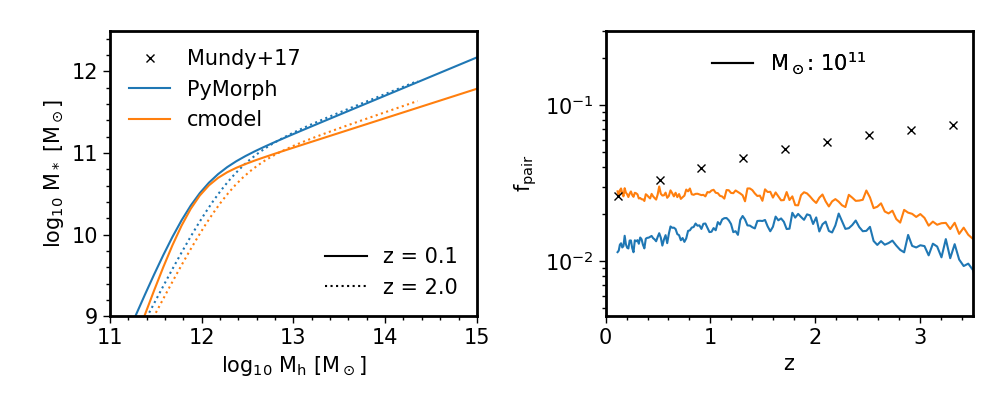
\includegraphics[width = \linewidth]{Figures/Chapter5/PairFractionData.png}
    \caption{Left: The stellar mass halo mass relations derived from PyMorph (blue) and cmodel (orange) at redshifts 0.1 (solid lines) and 2.0 (dotted lines). Right: The pair fraction evolution for galaxies using both SMHM relations. We make mass cuts, $>10^{10}M_{\odot}$ (dashed line) and $>10^{10}M_{\odot}$ (solid line), in PyMorph and cmodel. The black crosses show the corresponding best fits for the $>10^{11}M_{\odot}$ mass cut from \citet{Mundy2017A3.5}.}
	\label{fig:PairFractionData}
\end{figure*}

In an attempt to match the \citet{Mundy2017A3.5} pair fractions we begin using the cmodel SMHM relation which gives the closest match in pair fraction at low redshift. Following the analysis of Figure \ref{fig:PairFracSystematic} where higher $\gamma_{z}$ increases the pair fraction at high redshift we alter the parameter from 0.0 to 0.5 in steps of 0.1. In Figure \ref{fig:PairFractionHMevo} the left panel shows the SMHM relation at redshift 0.1 as a black dotted line then coloured lines show the relation at redshift $z = 2$ given the different $\gamma_{z}$ parameters. The right panel shows the impact of this evolution on the pair fraction, as predicted higher $\gamma_{z}$ increases the pair fraction with redshift and a value of above 0.1 removes the turnover. Comparing to \citet{Mundy2017A3.5} we see a value of $\gamma_{z}$ between 0.1 and 0.2 best reproduces the rise in pair fraction. 

\begin{figure*}
	\centering
	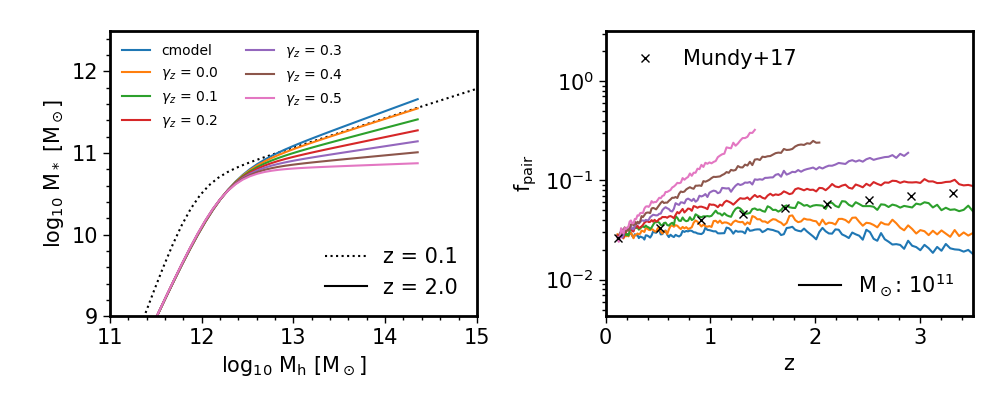
\includegraphics[width = \linewidth]{Figures/Chapter5/PairFractionHMevo.png}
    \caption{Left: The stellar mass halo mass relations derived from cmodel (black) at redshift $z = 0.1$ (dotted lines) and at $z = 2.0$ with altered high mass slope evolution parameter (coloured lines). Right: The pair fraction evolution for galaxies each altered SMHM relation in corresponding colour. The black crosses show the best fits for the $>10^{11}M_{\odot}$ mass cut from \citet{Mundy2017A3.5}.}
	\label{fig:PairFractionHMevo}
\end{figure*}

\section{Galaxy Morphologies Resulting from Galaxy Mergers}
%What happens during a galaxy merger?

Mergers are thought to be one of the drivers for morphological transformation, size growth and other galaxy changes \citep{Bournaud2007, Hopkins2009TheDemographics, Hopkins2010MergersFunctions, Shankar2011SizeUniverse, Fontanot2015OnMergers}. A number of analytically-based cosmological models have generally assumed that major mergers in particular, with a mass ratio of at least $M_{sat}/M_{cen} > 0.25(to 0.3)$, are effective in destroying disks and in forming ellipticals \citep{Baugh2006AApproach, Malbon2007BlackFormation, Bower2010TheFormation}. However, galaxy mergers happen on timescales that dwarf human lifespans so when we observe galaxy mergers we essentially see a static snapshot of the process. Therefore, much of our knowledge of galaxy mergers then comes from simulations of merging systems \cite[e..g.][]{Hopkins2006ASpheroids,Hopkins2009TheDemographics, Hopkins2010MergersRate,Hopkins2009HOWMERGERS,Hopkins2010MERGERSMATTER,OLeary2020EMERGE:zsim6,Fensch2017High-redshiftFormation,Stewart2008MergerSurvival,Stewart2009GALAXYDEPENDENCE}. 

Despite the wealth of simulations of galaxy mergers, the fulcrum of our understanding lies with the estimation of the rate and significance of mergers \cite{Hopkins2010MERGERSMATTER, Hopkins2010MergersRate}. Using the merger rates derived in Chapter \ref{Chapter:GalGrowth} we implement a post-processing method to ascertain the effects of traditional models when decoupled from merger trees and applied to true, statistical, populations in \steel.

%The fraction of elliptical galaxies stemming from galaxy major merger in steel
\subsection{Implementing discrete processes in a statistical model.}

One of the primary challenges in the development of \steel is trying to implement discrete processes in a statistical fashion. Mergers between two galaxies are implemented stochastically using the following method.
\begin{itemize}
    \item At each time-step for each central halo mass track the mass bins of previously accreted subhalo/satellite galaxy mass functions that have reached the end of their dynamical time are summed to produce the merging satellite stellar mass function. 
    \item Each central halo mass track is assigned a central stellar mass at each epoch $M_{*,cent}(M_{h}, z)$ (Figure \ref{fig:Cent_Mass_PP}). By integrating the merging satellite stellar mass function in the range [$M_{*,cent}(M_{h}, z) \cdot \mu$, $M_{*,cent}(M_{h}, z)$] the probability that a given central has undergone a major merger at each epoch is retrieved, where $\mu$ is the major merger mass ratio. 
    \item In Figure \ref{fig:Gal_Morph_toon} an illustration of the way galaxy morphologies are updated is given. 
    \begin{itemize}
        \item In the leftmost panel all galaxies are spirals or a disk like morphology (blue bar), the probability of a galaxy having a major merger is shown as a black line.
        \item Following the arrow to the middle panel the fraction of galaxies that had a major merger are assigned as ellipticals. The mass track at this epoch now has this spiral to elliptical ratio.
        \item At this next time step the fraction of galaxies undergoing a major merger is calculated, however, this is split between galaxies that have previously had a major merger and those that have not. 
        \item Following the arrow from the middle to the right hand panel we see only the galaxies that were in the spiral group contribute to the increased elliptical fraction.
        \item Using this process at each time-step eventually all galaxies can become elliptical but the rate at which this happens slows due to the decreasing spiral population.
    \end{itemize}
\end{itemize}

\begin{figure}[h]
	\centering
	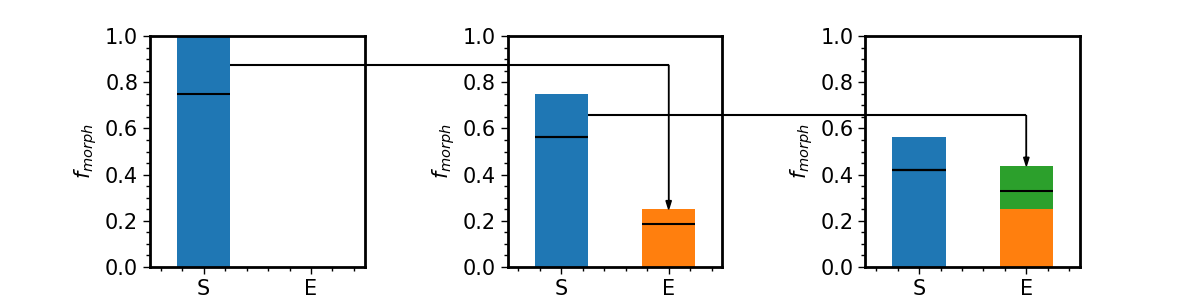
\includegraphics[width = \linewidth]{Figures/Chapter5/Morphology_Evolution.png}
	\caption{A cartoon to show the way we assign morphologies statistically in $\steel$. Each step has the same fraction of major mergers but the number of ellipticals created reduces as some major mergers occur on the elliptical fraction. The fraction of galaxies in each population experiencing a major merger is displayed as a horizontal black line.}
	\label{fig:Gal_Morph_toon}
\end{figure}

Applying the above process to galaxies in \steel from redshift $z = 3$ we obtain the morphological fraction of galaxies at different masses using a major mass ratio of $\mu = 0.25$, at redshifts $z = 0.1, 0.65, 1.75$. Figure \ref{fig:Gal_Morph} shows the probability/fraction of central galaxies that have elliptical morphologies, while the black triangles show the T-Type-selected elliptical fraction from the SDSS catalogue at redshift $z = 0.1$. We find that applying this simple recipe to the merging number densities from \textsc{steel} creates a good match to the elliptical fraction in the local universe.

\begin{figure}[h]
	\centering
	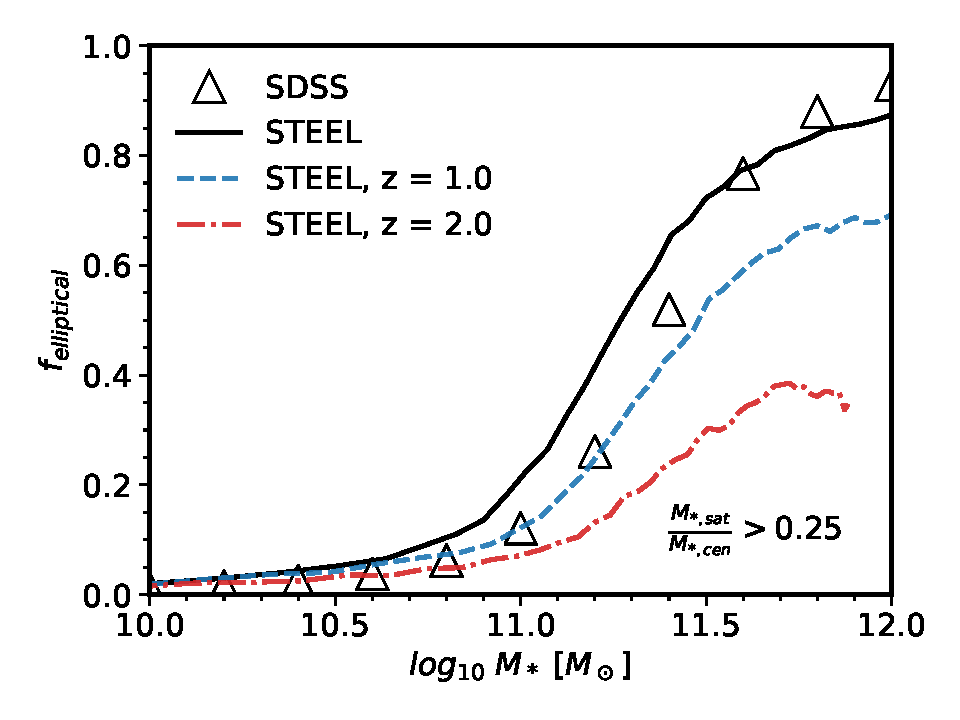
\includegraphics[width = \linewidth]{Figures/Chapter5/GalaxyMorphologies.pdf}
	\caption{We show at three redshift steps the predicted fraction of ellipticals as a function of stellar mass. The lines are the predictions from \textsc{steel} and the triangles are the T-Type selected elliptical fraction from SDSS at redshift $z = 0.1$.}
	\label{fig:Gal_Morph}
\end{figure}


\section{Lenticular Galaxy Formation}
%What is a lenticular and why are they considered independently to the rest of the galaxy population?
Lenticular galaxies are categorised by their unusual appearance, in the famous `tuning fork' diagram derived from \citet{Hubble1927TheNebulae} the lenticular galaxies are found where the two spiral `forks' meet the elliptical `handle'. Lenticulars similar to spirals have an extended disk but do not boast the `bars' or `arms' that decorate the disks of spiral galaxies nor the resiviors of cold gas suitable for star formation \cite{CHAMARAUX1986TheSamples}; similar to ellipticals lenticulars have a velocity dispersion dominated bugle at their centre. 
%What have been the proposed models of Lenticular formation?

Given that lenticulars sit between and share properties of both the other types of galaxy it is reasonable to think that they could exist on the transformation pathway between the two populations. This finding is potentially supported given lenticulars are preferentially found in the cluster environment \cite{Dressler1980GalaxyGalaxies} and the fraction of lenticulars increases with decreasing redshift simmilar to that of ellipticals \cite{Postman2005TheClusters}. 

%Building a least assumption model of lenticular formation (supervised project)
\subsection{Lenticular formation in empirically constrained environments.}
\textit{The work presented in this subsection was carried out by SP under the supervision of PJG and FS. The direction of the project was heavily influenced by PJG and builds upon the successes found in predicting morphologies in \steel.}

Given the successes in ratifying the simple merger model of elliptical formation within \steel, we use several literature suggested models of lenticular formation to build a `minimal assumption' model that fits the morphological fractions from SDSS.

\subsubsection{\citet{Cook2009Two-phaseFormation} Model}

We started our investigation by implementing the lenticular formation model from \citet{Cook2009Two-phaseFormation}. This model divides halo growth into two distinct phases, a fast collapse and intense merging phase at high redshift, and a slow accretion low redshift phase after a transition epoch $z_{t}$. The galaxy growth related to this two phase halo growth is that the spheriod forms at high redshift and the disk at low redshift. The model for building spheorids in this semi-analytic model is the same as that implemented in \citet{Granato2004AHosts}. 

Translating semi-analytical techniques into a semi-empirical model by nature of the two models results in a loss of complexity, to distil this model we focus on the two phase formation. Galaxies are selected where they have grown a significant fraction of their mass (e.g. 70\%) between two epochs as assigned as lenticulars. These galaxies can then undergo further evolution by being transformed into ellipticals as described by the merger model from the previous section. Despite utilising complete freedom in the mass fraction required and redshift thresholds we find that within the framework given by \steel this model can not reproduce the lenticular fractions as illustrated by the results shown in Figure \ref{fig:CookeModel}.

\begin{figure}
  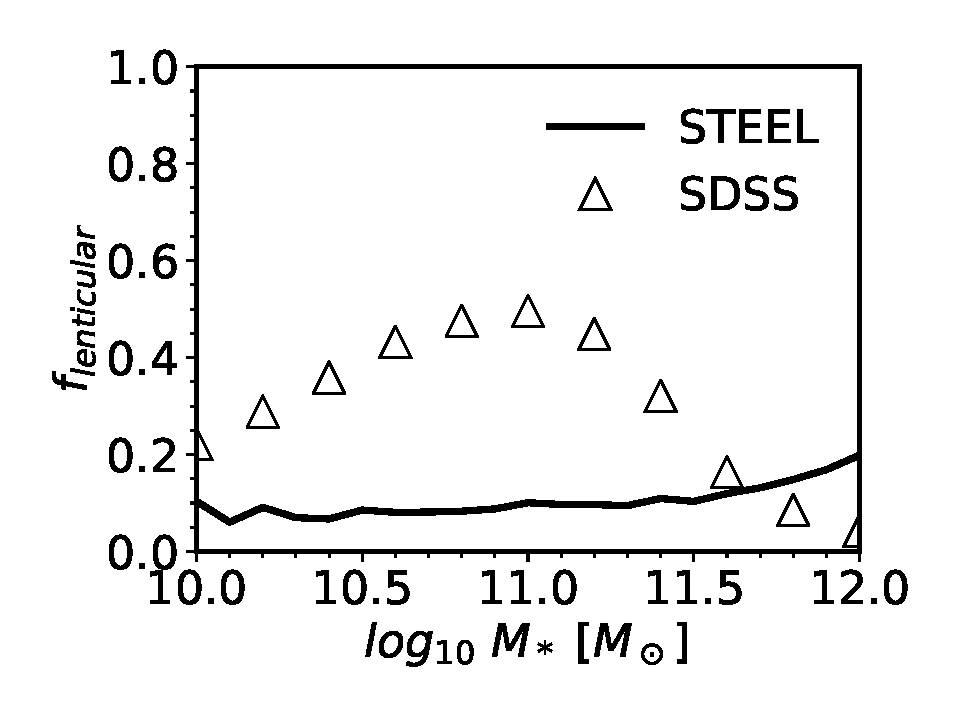
\includegraphics[width=\linewidth]{Figures/Chapter5/CookModel.pdf}
    \caption{Lenticular galaxy fractions generated using a very simplified
      version of the lenticular formation method described in
      \cite{Cook2009Two-phaseFormation}. The model assumes lenticular galaxies are those that have formed a significant fraction of their mass during a particular epoch. However, even after significant optimisation of the mass
      threshold and epoch definitions, it is not possible to reproduce the SDSS
      data within \steel using this model.}
    \label{fig:CookeModel}
\end{figure}

\subsubsection{Minimal assumption model}

Given the unsuccessful implementation of the \citet{Cook2009Two-phaseFormation} model we revisit other literature proposed models to find out which (or combination of which) have the potential to generate the observed lenticular fraction. Considering the nature of lenticulars in observations which increase their fraction with decreasing redshift in a similar fashion to ellipticals the first model we implement extends that of the elliptical merger model. An additional merger mass threshold ($\mu$) is implemented at $\mu = M_{*, sat}/M_{*, cen} = 0.05$. Central galaxies that experience a merger between this mass threshold and the major merger threshold are assigned to be lenticulars. Lenticular galaxies that then experience mergers above the ratio are reassigned as ellpticals. This essentially adds a central 3rd column to Figure \ref{fig:Gal_Morph_toon}. As can be seen in the first panel of \ref{fig:Lentcular_panels} this simplistic model over produces lenticulars in the high mass end. 

To reduce the lenticular production at high masses, following simmilar ideas to the gas dissipation models utilised in \citet{Hopkins2009} we test a hard gas threshold. Physically this gas threshold can be interpreted as a damping force, the gas dissipates the energy of the merger into heating the gas reservoir limiting the disruption to the galaxy structures. Initially only galaxies with a gas fraction above the threshold can be converted into lenticulars, as shown in the middle panel this removes all lenticulars from the high mass end where galaxies tend to be gas poor. 
Finally, to improve the fit a soft gas fraction is implemented where galaxies below a given mass fraction become statistically less likely to become lenticulars after experiencing a major merger. We include the soft gas threshold to reflect the varying efficiency of gas at different fractions dissipating the energy. This combination of models well fits the high mass lenticulars as can be seen in the rightmost panel of Figure \ref{fig:Lentcular_panels}.

\begin{figure}
  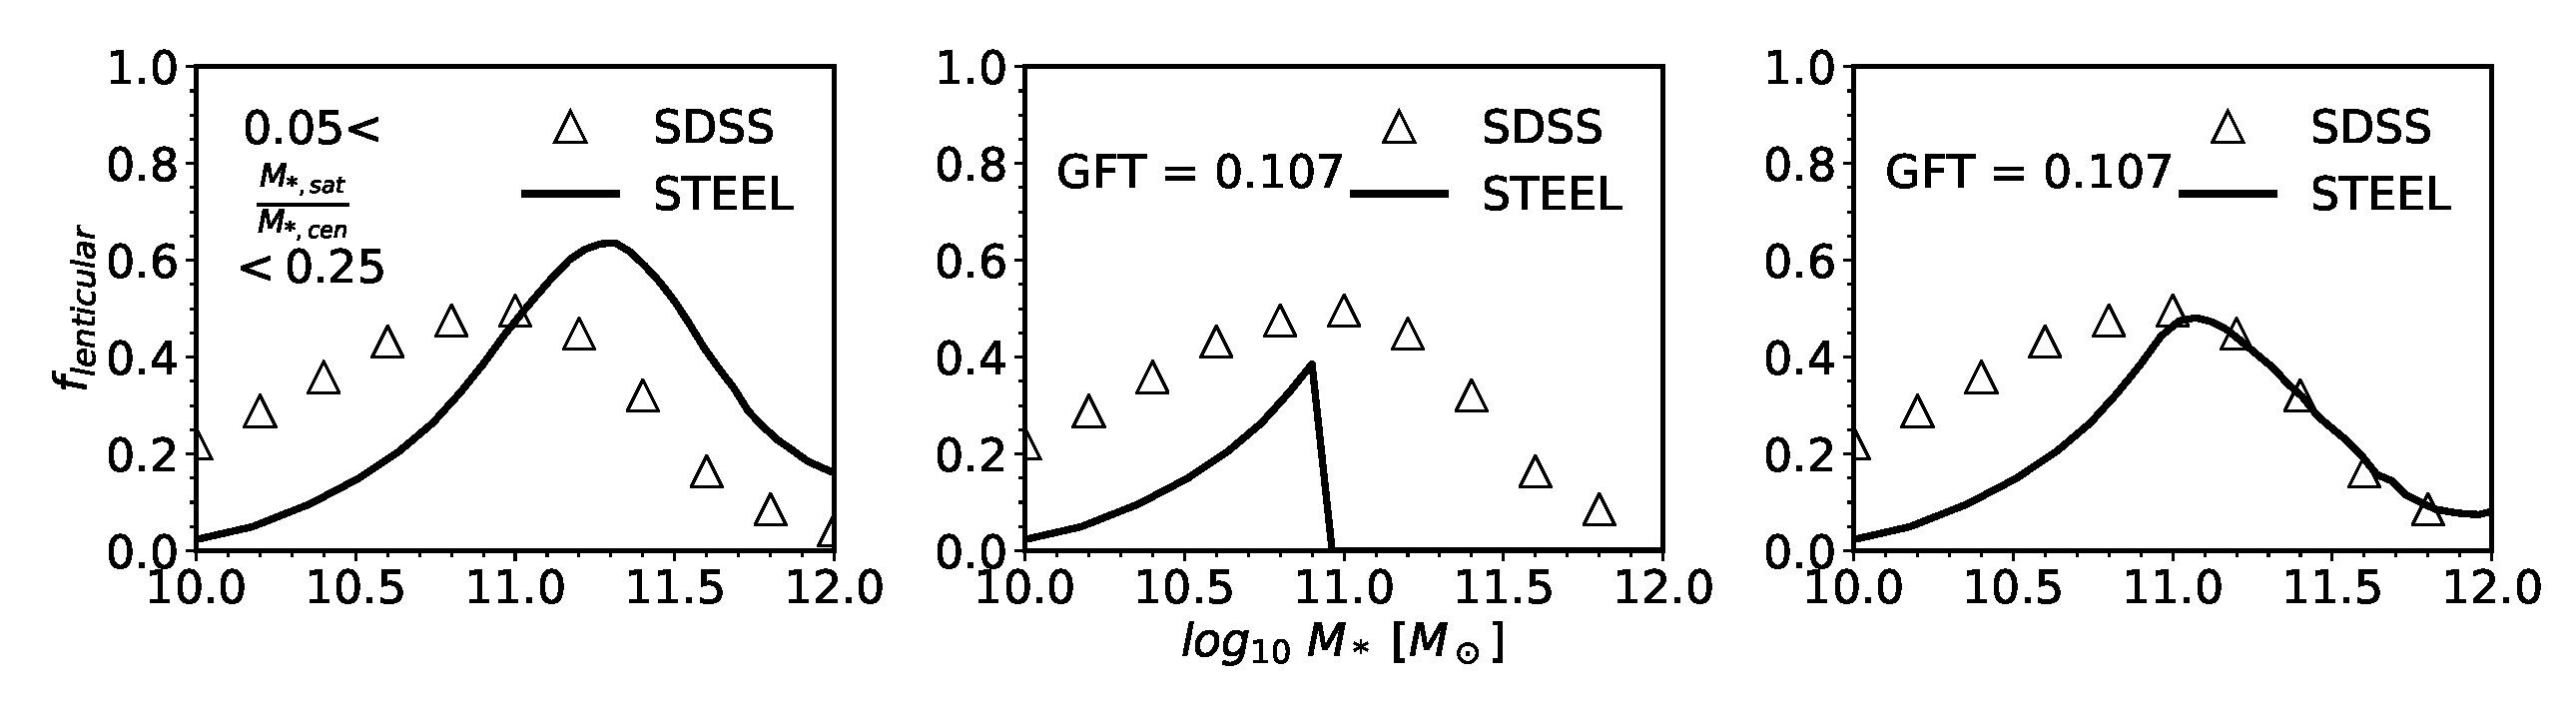
\includegraphics[width=\linewidth]{Figures/Chapter5/Lenticular_three.pdf}
    \caption{Three plots from left to right show lenticular fractions generated using the progressive development of the lenticular merger model. The first (leftmost) panel shows the fraction generated by summing the number densities of merging galaxies with mass ratio in the range $0.05 < \mu < 0.25$. The middle panel shows the effect of adding a hard gas ratio cutoff to the merger model, galaxies that are above a gas fraction threshold (GFT) do not form lenticulars. Finally, changing the model to a `soft' gas fraction threshold where the efficiency of lenticular formation is reduced above the GFT.}
    \label{fig:Lentcular_panels}
\end{figure}

Lower mass galaxies reside in less rich environments and grow more via secular (in-situ) processes, it is therefore understandable that the merger/dissipation model does not make lenticulars at these masses.

To build lenticulars at these masses we implement a disk instability model following the baryonic inflow rates given by \citet{Bournaud2011BLACKSTREAMS}. Applied along the accretion histories we allow galaxies to build their central bulges though gas transport from the disk using Equation \ref{eqn:DiskInflow}, 

\begin{equation}
    \label{eqn:DiskInflow}
    \dot{M}_{inflow} = 25 log_{10}\Big[\frac{M_{*,disk}}{10^{11}}\Big]\Big(\frac{1 + z}{3}\Big)^{1.5},
\end{equation}

the mass of the bulge is then given by,

\begin{equation}
    M_{bulge} = \sum_z \dot{M}_{inflow} \times \delta t(z),
\end{equation}

in each mass bin a fraction of galaxys proportional to the mass ratio of the bulge to the total stellar mass, $A \times M_{bulge} / M_{*, total}$, is added to the lenticular population. The resulting fit to the population is shown in Figure \ref{fig:All_Morphologies}.

\begin{figure}
  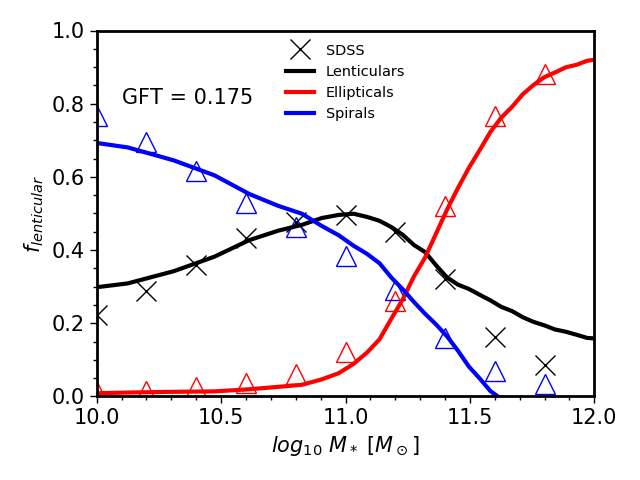
\includegraphics[width=\linewidth]{Figures/Chapter5/Bulge_Growth_Final_All_Morph.png}
    \caption{We show the fractions of morphologies as a function of mass. Ellipticals are generated using a major merger model, lenticulars using the combined merger (with soft gas fraction) and baryonic inflow models} and, spirals are the remaining population.
    \label{fig:All_Morphologies}
\end{figure}

We find the combination of a merger and inflow model is able to adequately recreate the lenticular fractions. This two model fit is potentially consistent with the distinct morphological types, barred and un-barred found within the lenticular population \cite{Laurikainen2005MulticomponentGalaxies, VanDenBergh2012LuminositiesGalaxies}.

In summary, to recreate the lenticular population we find it necessary to add three parameters in addition to the major merger mass ratio used to create the ellipticals. The first is the `minor' mass ratio limit that defines the minimium mass ratio at which lenticulars are formed via mergers, the second the is the `soft' gas mass threshold that damps the creation of lenticulars and, finally the parameter to convert the bulge ratios to lenticular fraction. 

\section{Discussion}

In this chapter we have shown two applications of \steel. Firstly is the ability of \steel to unravel the effects of systematics in galaxy observables using the galactic pair fractions. Secondly, we show an example of how constrained merger histories can be used to test if proposed morphological evolution models recreate the observed morphological fractions.  

\subsection{Pair Fractions}

The primary goal of the pair fraction analysis is to show the propagation of systematics in galaxy modelling. 
Specifically, we use the SMHM relationship to connect assumptions used when estimating stellar masses from observations to systematics in galaxy pair fractions in the context of a \LCDM Universe. 
In this chapter we have used two observed stellar mass functions from SDSS-DR7 observations that use a de Vaucoulers and a S\`ersic + Exponential fit to determine stellar masses, which in turn generate stellar mass functions with notably different number densities at the high mass end. Each stellar mass function then generates, through abundance matching, a different SMHM relationship. The S\`ersic + Exponential mass function generates a steeper high-mass slope in the SMHM relationship at any epoch.
In addition to the SMHM relationships from the observed data we use a relationship fitted to match the outputs of the Illistris simulation. Furthermore, we also consider a toy model SMHM relation individually perturbing each input parameter to transparently probe the impact of the input SMHM relation on the pair fractions.
In each case we find that small changes introduced into the SMHM relationship can have significant effects on the expected pair fractions, as shown in Figures \ref{fig:MassRatioCartoon},\ref{fig:SMHM_PF_Cartoon}, \& \ref{fig:PairFracSystematic}.
This suggests that in the contxet of a \LCDM Universe tensions in previous observational studies could, in large part, be traced back to systematics in stellar mass estimates.

In \citet{Mundy2017A3.5} the $M_{*,cen} > 10^{10} M_{\odot}$ pair fraction is given, however, this is not significantly different from the $M_{*,cen} > 10^{11} M_{\odot}$ pair fraction shown in Figure \ref{fig:PairFractionData}. In Figure \ref{fig:PairFracSystematic} we find the pair fraction drops significantly when mass a selection is taken below the SMHM relation knee. As this drop is not found by \citet{Mundy2017A3.5} we interpret that their pair fraction measurement is not consistent with a break in the SMHM relation between $10^{10} M_{*,cen}$ and $10^{11} M_{*,cen}$.

\citet{Man2016RESOLVING03} noticed that the choice between luminosity-selected and stellar-mass selected pairs affected the pair fraction evolution. In this work we have provided a clear framework to properly interpret how input choices create systematic effects in the observed pair fraction and its evolution. Furthermore, it is a common approach to infer the assembly history of galaxies by converting the pair fractions into merger rates by assigning timescales to galaxy pairs \citep{Conselice2003A3,Conselice2008TheField,Mundy2017A3.5}. 
In \Paper{2} we developed a model that calculates the stellar mass growth rates of central galaxies and the stellar mass accretion rate from satellite galaxies.
It is found that, for some SMHM relationships, the accretion rate can be greater than the total growth rate implying the model is internally inconsistent and the SMHM relationship is not compatible with this \LCDM cosmology.
The stellar mass accretion rate is connected to the merger frequency and therefore the galaxy pair fraction. 
In this work we connect the shape and evolution of the SMHM relationship to the evolution of the pair fractions.
We propose it is therefore possible to use the pair fraction as an additional constraint to the SMHM relationship, this is a natural extension of conditional abundance matching or extended SHAM (subhalo abundance matching) models \citep{Hearin2013SHAMGroups}.
Using \steel one can test simultaneously the accretion ratio and the pair fraction generated from a given stellar mass function and cosmology.

Any changes to the stellar mass estimates such as photometry, background subtraction, IMF, e.t.c. that affect the stellar mass function will in a given cosmology create a change in the SMHM relationship. Therefore by the systematic propagation demonstrated in this work any stellar mass estimation will create systematic differences in the pair fractions. 
With the techniques presented throughout this thesis, one could retrieve the systematic differences created in pair fraction under multiple \LCDM cosmologies and for any given set of stellar mass functions. As a further test of our results we show the pair fractions found in Illustris, together with the pair fractions predicted by \steel, using a SMHM relationship designed to match
that of Illustris are fully consistent.

In the era of wide and deep surveys, such as EUCLID, constraining a model using a single multi-epoch data set with consistent photometry will become a reality. The advantages of this are twofold: By tuning the SMHM relation to a given survey over a large range of redshifts the growth of the stellar mass function over time can be tested against the implied satellite accretion and star formation rate as in Chapter \ref{Chapter:GalGrowth} this can be seen as a test of the consistency of the cosmological model or of the consistency of the stellar mass and/or starformation rate estimation. Secondly, as in Chapter \ref{Chapter:GalDist} one can test if the high redshift SMHM relation is consistent with the low redshift satellite distributions. The constraints on a given photometry, cosmological model, satellite evolution, starformation rate, e.t.c... are still not complete however it will allow nonphysical results to be identified. Furthermore, by making the model accessible it can then be used in the manner described above to make systematic adjustments to compare between current and future data sets that may use different stellar mass estimations.

\subsection{Morphologies}

Given the very promising results of \steel in predicting satellite number densities in different environments and epochs, we here take a step further and explore whether \steel's cumulative number of major mergers is able to account for the local fraction of elliptical galaxies as well as implementing several literature inspired lenticular formation models. 

Despite the noticeably good agreement between model predictions and data in Figure \ref{fig:All_Morphologies}, we stress that different input SMHM relations can, as shown in this Chapter \ref{Chapter:GalGrowth}, substantially affect the accretion rate which in turn will modify the number of galaxies experiencing major mergers. It follows that any cosmological galaxy evolution model that uses mergers as a physical driver for galaxy transformation should first simultaneously and self-consistently closely reproduce stellar mass functions, the SMHM relation, satellite distributions, and pair fractions at previous redshifts.

\section{Conclusions}
\label{sec:Conclusions}

In the first part of this Chapter, we show that the input SMHM relations, based on different stellar mass estimations, have a significant impact on the predicted galaxy pair fraction. In short, the steeper the relation, the lower the pair fraction. Specifically we compare stellar mass functions created with a de Vaucoulers-based photometry (cmodel) to a S\'ersic-Exponential photometry (PyMorph), the latter leading to an enhancement in the number density of high mass galaxies. The resulting effect of these stellar mass functions is a different input SMHM relation to $\steel$, the primary difference consisting of a steeper high mass slope when adopting the S\'ersic-Exponential profile. As expected, the S\'ersic-Exponential results in a lower pair-fraction. To attempt to explain the difference in pair-fraction evolution with redshift we create a suite of toy models testing different alterations to the SMHM relation. We find that this evolution is linked to the evolution of the high mass slope.

The purpose of this work is to show how subtle changes in derivation of stellar mass could lead to large differences in the pair fraction observed. It is therefore crucial when comparing two different samples to account for the systematic biases introduced by the assumptions implicit in stellar mass estimation as shown in this work to avoid systematic effects from a simulations foundation propagating to more `delicate' physics or driving unwanted feedback processes.

The second part of this Chapter shows how the implementation of simple morphological models into \steel allows for analysis of said models expected outcome on the full galaxy population. We show that the major merger model well reproduces the observed distributions. Whereas, the Cook model for lenticular formation does not well reproduce the morphological fractions. This ability to flexibly add models without the need to substantially alter the core of the simulation is what lends semi-empirical models their transparency. We then use this transparency to build a `least assumption' model where it is clear what each modelling assumption does to the morphological fractions.

In conclusion, future surveys should look to use fast and flexible modelling alongside data products to be able to properly understand the systematic effects of assumptions made on derived data products. For example the SMHM relation must simultaneously fit: traditional abundance matching, self-consistency between satellite accretion and central galaxy growth, and as shown in this paper the normalisation and evolution of the galaxy pair fraction. This multi-product fitting will ensure relations such as the SMHM relation are not only better constrained but can also be co-constrained with other observables. In addition to this \steel provides a platform that combines fast development and running to test formation models in to make iteration of theoretical models more practical. In these developments we see how the design principles fundamental to \steel as laid out in Chapter \ref{Chapter:Method} begin to pay dividends.
